\chapter{Pakej Arab\TeX{} dan \emph{alqalam}}

\section{Arab\TeX{}}

Secara asasnya, sepanjang yang penulis ketahui tulisan Arab di dalam Arab\TeX{} dihasilkan menggunakan huruf-huruf Roman seperti berikut:\\

\begin{minipage}{\linewidth}
%\begin{figure}[h!tb]
\begin{center}
\begin{tabular}{|c|c|c|c|c|c|c|c|c|c|c|c|c|c|}
\hline
\rule[-6pt]{0pt}{16pt}
<A> & <b> & <t> & <_t> & <j> & <.h> & <_h> &
<d> & <_d> & <r> & <z> & <s> & <^s> & <.s> \\
\hline
\verb#A# & \verb#b# & \verb#t# & \verb#_t# & \verb#j# & \verb#.h# & \verb#_h# &
\verb#d# & \verb#_d# & \verb#r# & \verb#z# & \verb#s# & \verb#^s# & \verb#.s#\\
\hline
\hline
\rule[-7pt]{0pt}{17pt}
<.d> & <.t> & <.z> & <`> & <.g> & <f> & <q> &
<k> & <l> & <m> & <n> & <h> & <w> & <y> \\
\hline
\verb#.d# & \verb#.t# & \verb#.z# & \verb#`# & \verb#.g# & \verb#f# & \verb#q# &
\verb#k# & \verb#l# & \verb#m# & \verb#n# & \verb#h# & \verb#w# & \verb#y# \\
\hline
\end{tabular}
\end{center}
\end{minipage}\\

Huruf asing, yang bukan Arab:\\
\bigskip
\begin{minipage}{\linewidth}
\begin{center}
\begin{tabular}{|c|c|c|c|c|c|c|c|c|c|}
\hline
<p> & <v> & <^c> & <,c> & <^z> & <g> & <c> & <^n> & <^l> & <.r> \\
\hline
\verb#p# & \verb#v# & \verb#^c# & \verb#,c# & \verb#^z# & \verb#g# &
\verb#c# & \verb#^n# & \verb#^l# & \verb#.r# \\
\hline
\end{tabular}
\end{center}
\captionof{figure}{Susunatur huruf dan bagaimana untuk anda tulis di dalam teks Arab\TeX{}}%\cite{paut-arab}}
%\footnote{http://www.win.tue.nl/~aeb/natlang/arabic/arabtex-verb-doc.html}}
\label{arab-rujuk}
%\end{figure}
\end{minipage}

Jadual \ref{arab-rujuk} ini turut memaparkan bagaimana untuk anda menulis Jawi di dalam Arab\TeX{} yang diambil dari sumber asalnya (lihat nombor rujukan di bahagian belakang buku ini)\cite{paut-arab}.


\section{\emph{alqalam}}
Pakej ini membolehkan anda memasukkan teks al-quran, atau mencetak teks al-quran di dalam tulisan anda.
Kita tengok contoh kod yang dimuatkan di dalam sampel dari dokumentasi alqalam. Surah yang dipaparkan berikut merupakan sebahagian ayat dari
Surah as Sajadah, kod sumber \latex{} boleh dimuat turun di laman mirror Debian untuk alqalam.%\footnote{http://ftp.de.debian.org/debian/pool/main/a/alqalam/alqalam\_0.2.orig.tar.gz}
\cite{paut-kalam}.
%\lstset{inputencoding=utf8x, extendedchars=\true}
%
%\begin{Verbatim}[frame=single]
%\end{Verbatim}

%\lstinputlisting{sajda.tex}


%\begin{landscape}
%\begin{multicols}{2}
%\begin{minipage}{0.25\linewidth}
\begin{minipage}{\linewidth}
\begin{center}

%\fbox{
%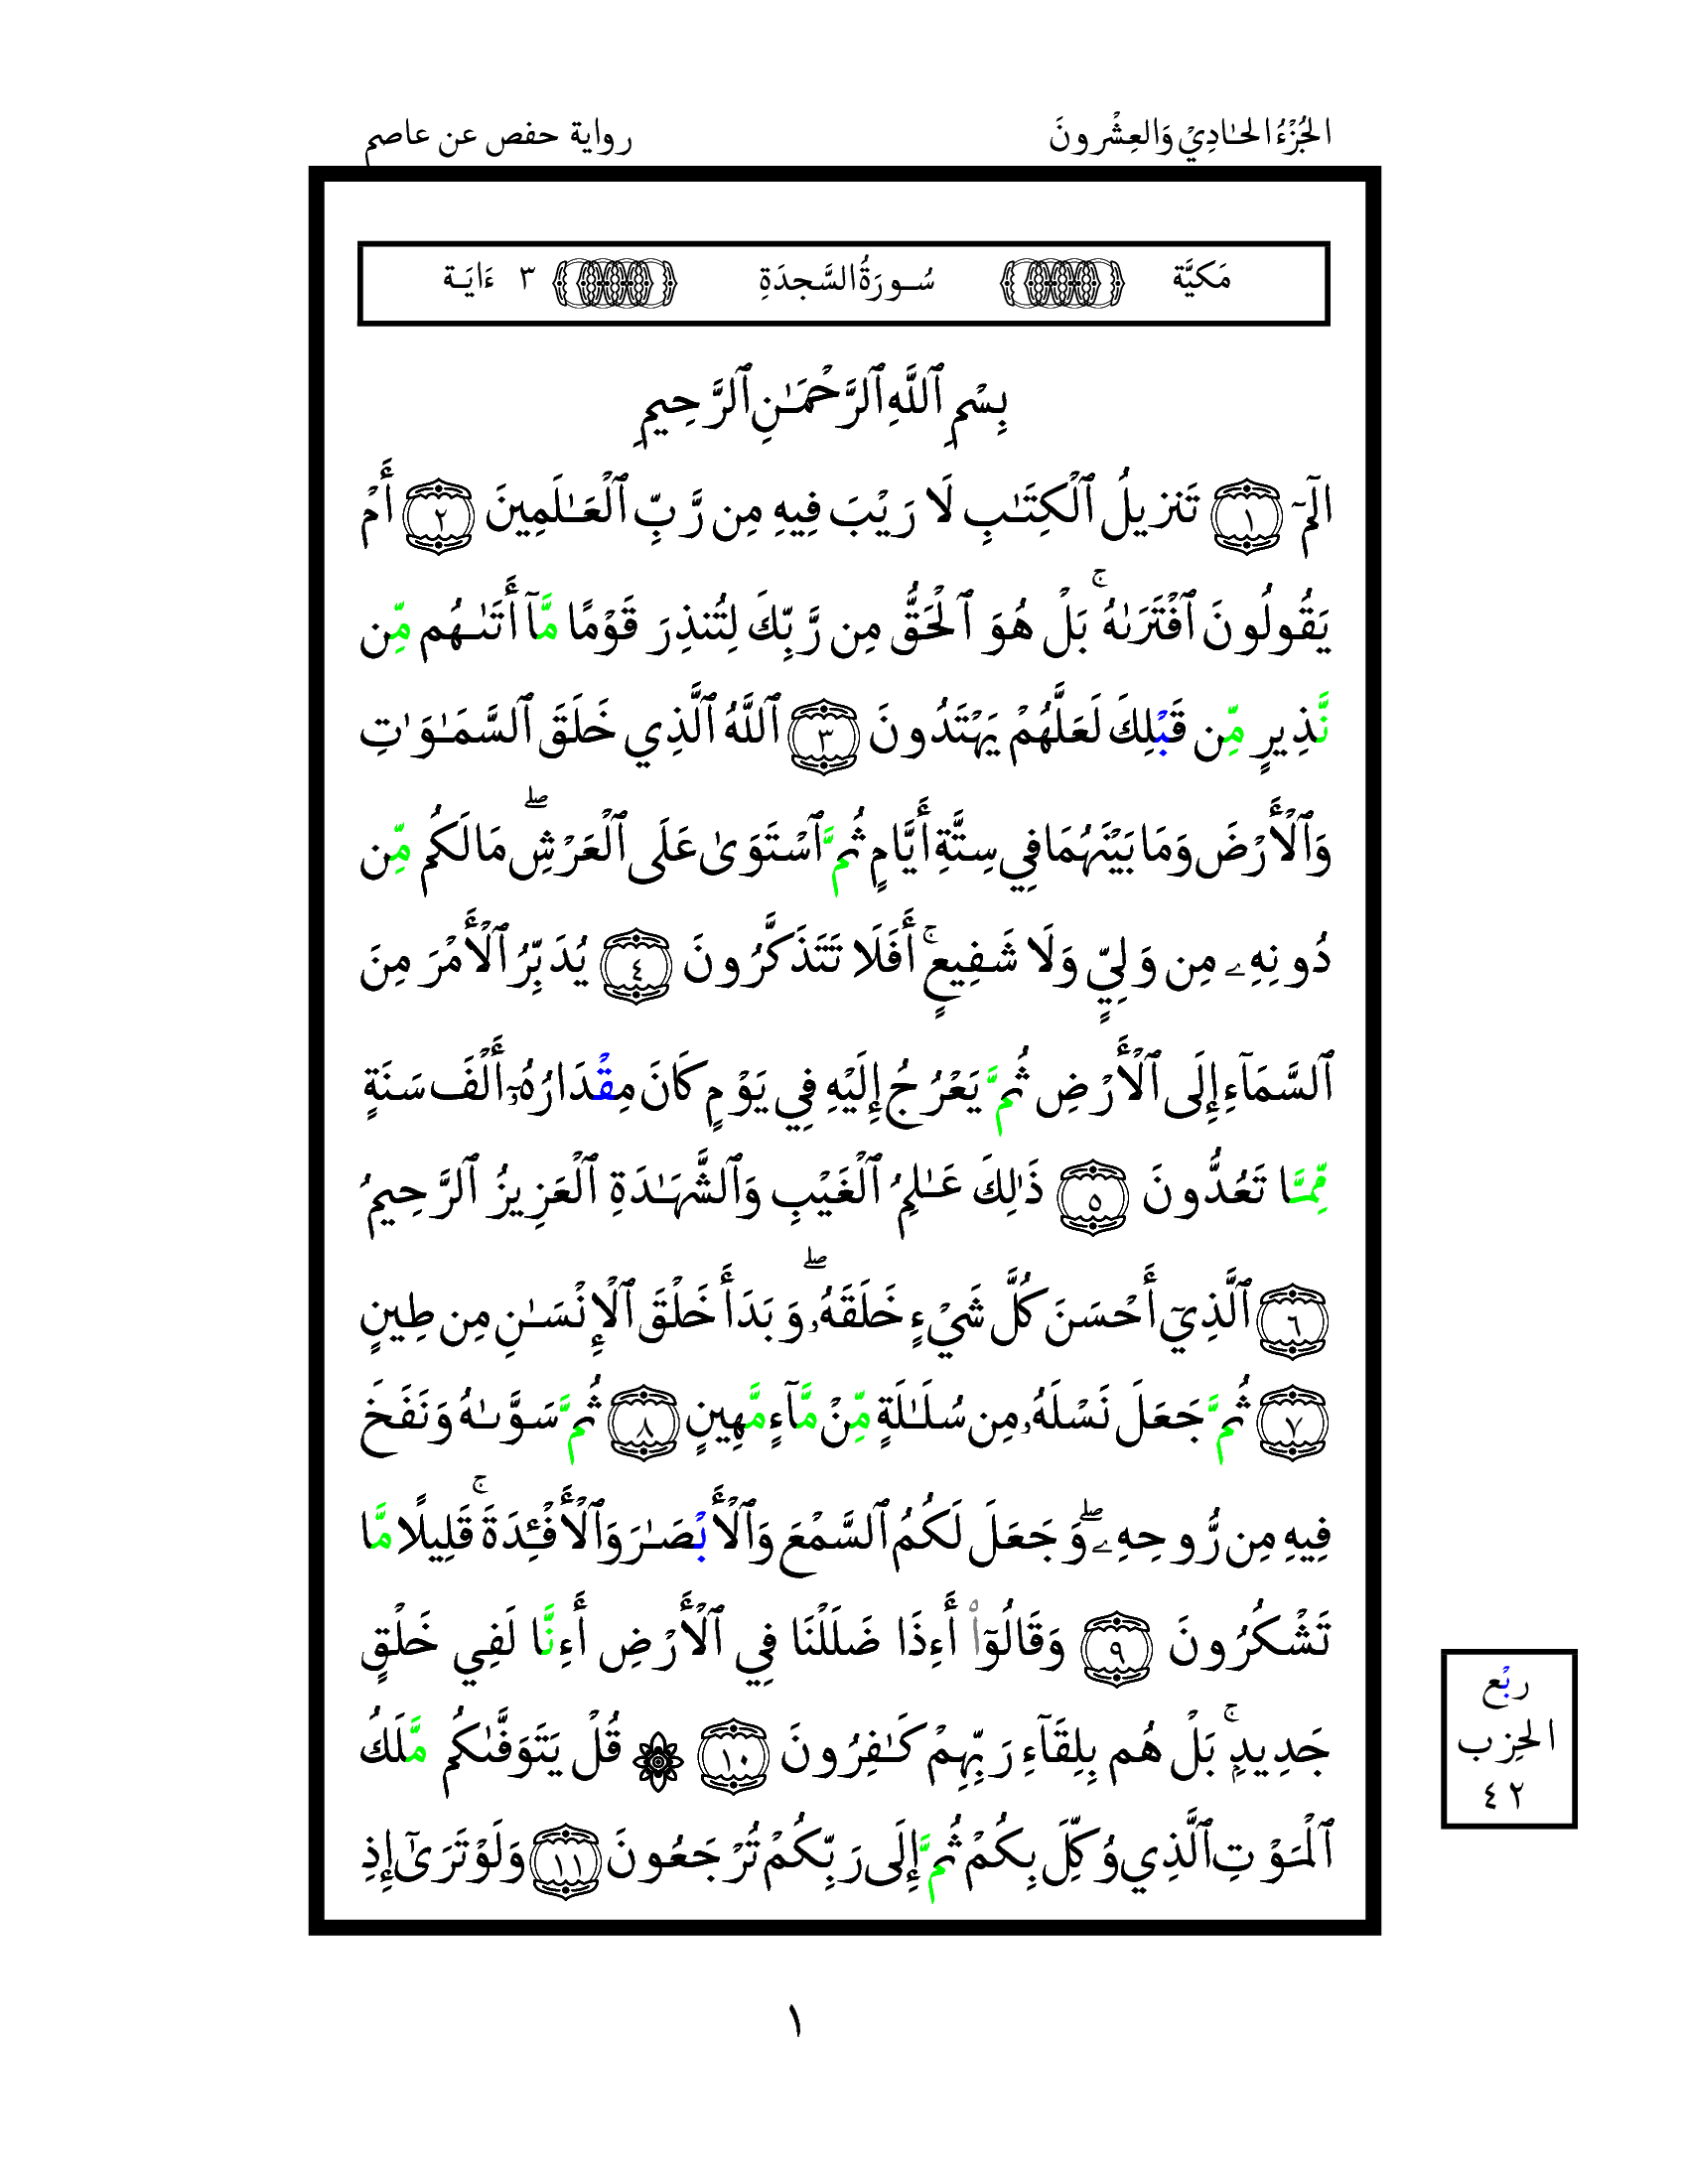
\includegraphics[scale=0.6]{sajdah_1.png}
%}
\end{center}
\end{minipage}

%\begin{minipage}{1\linewidth}
%\begin{center}
%\fbox{
%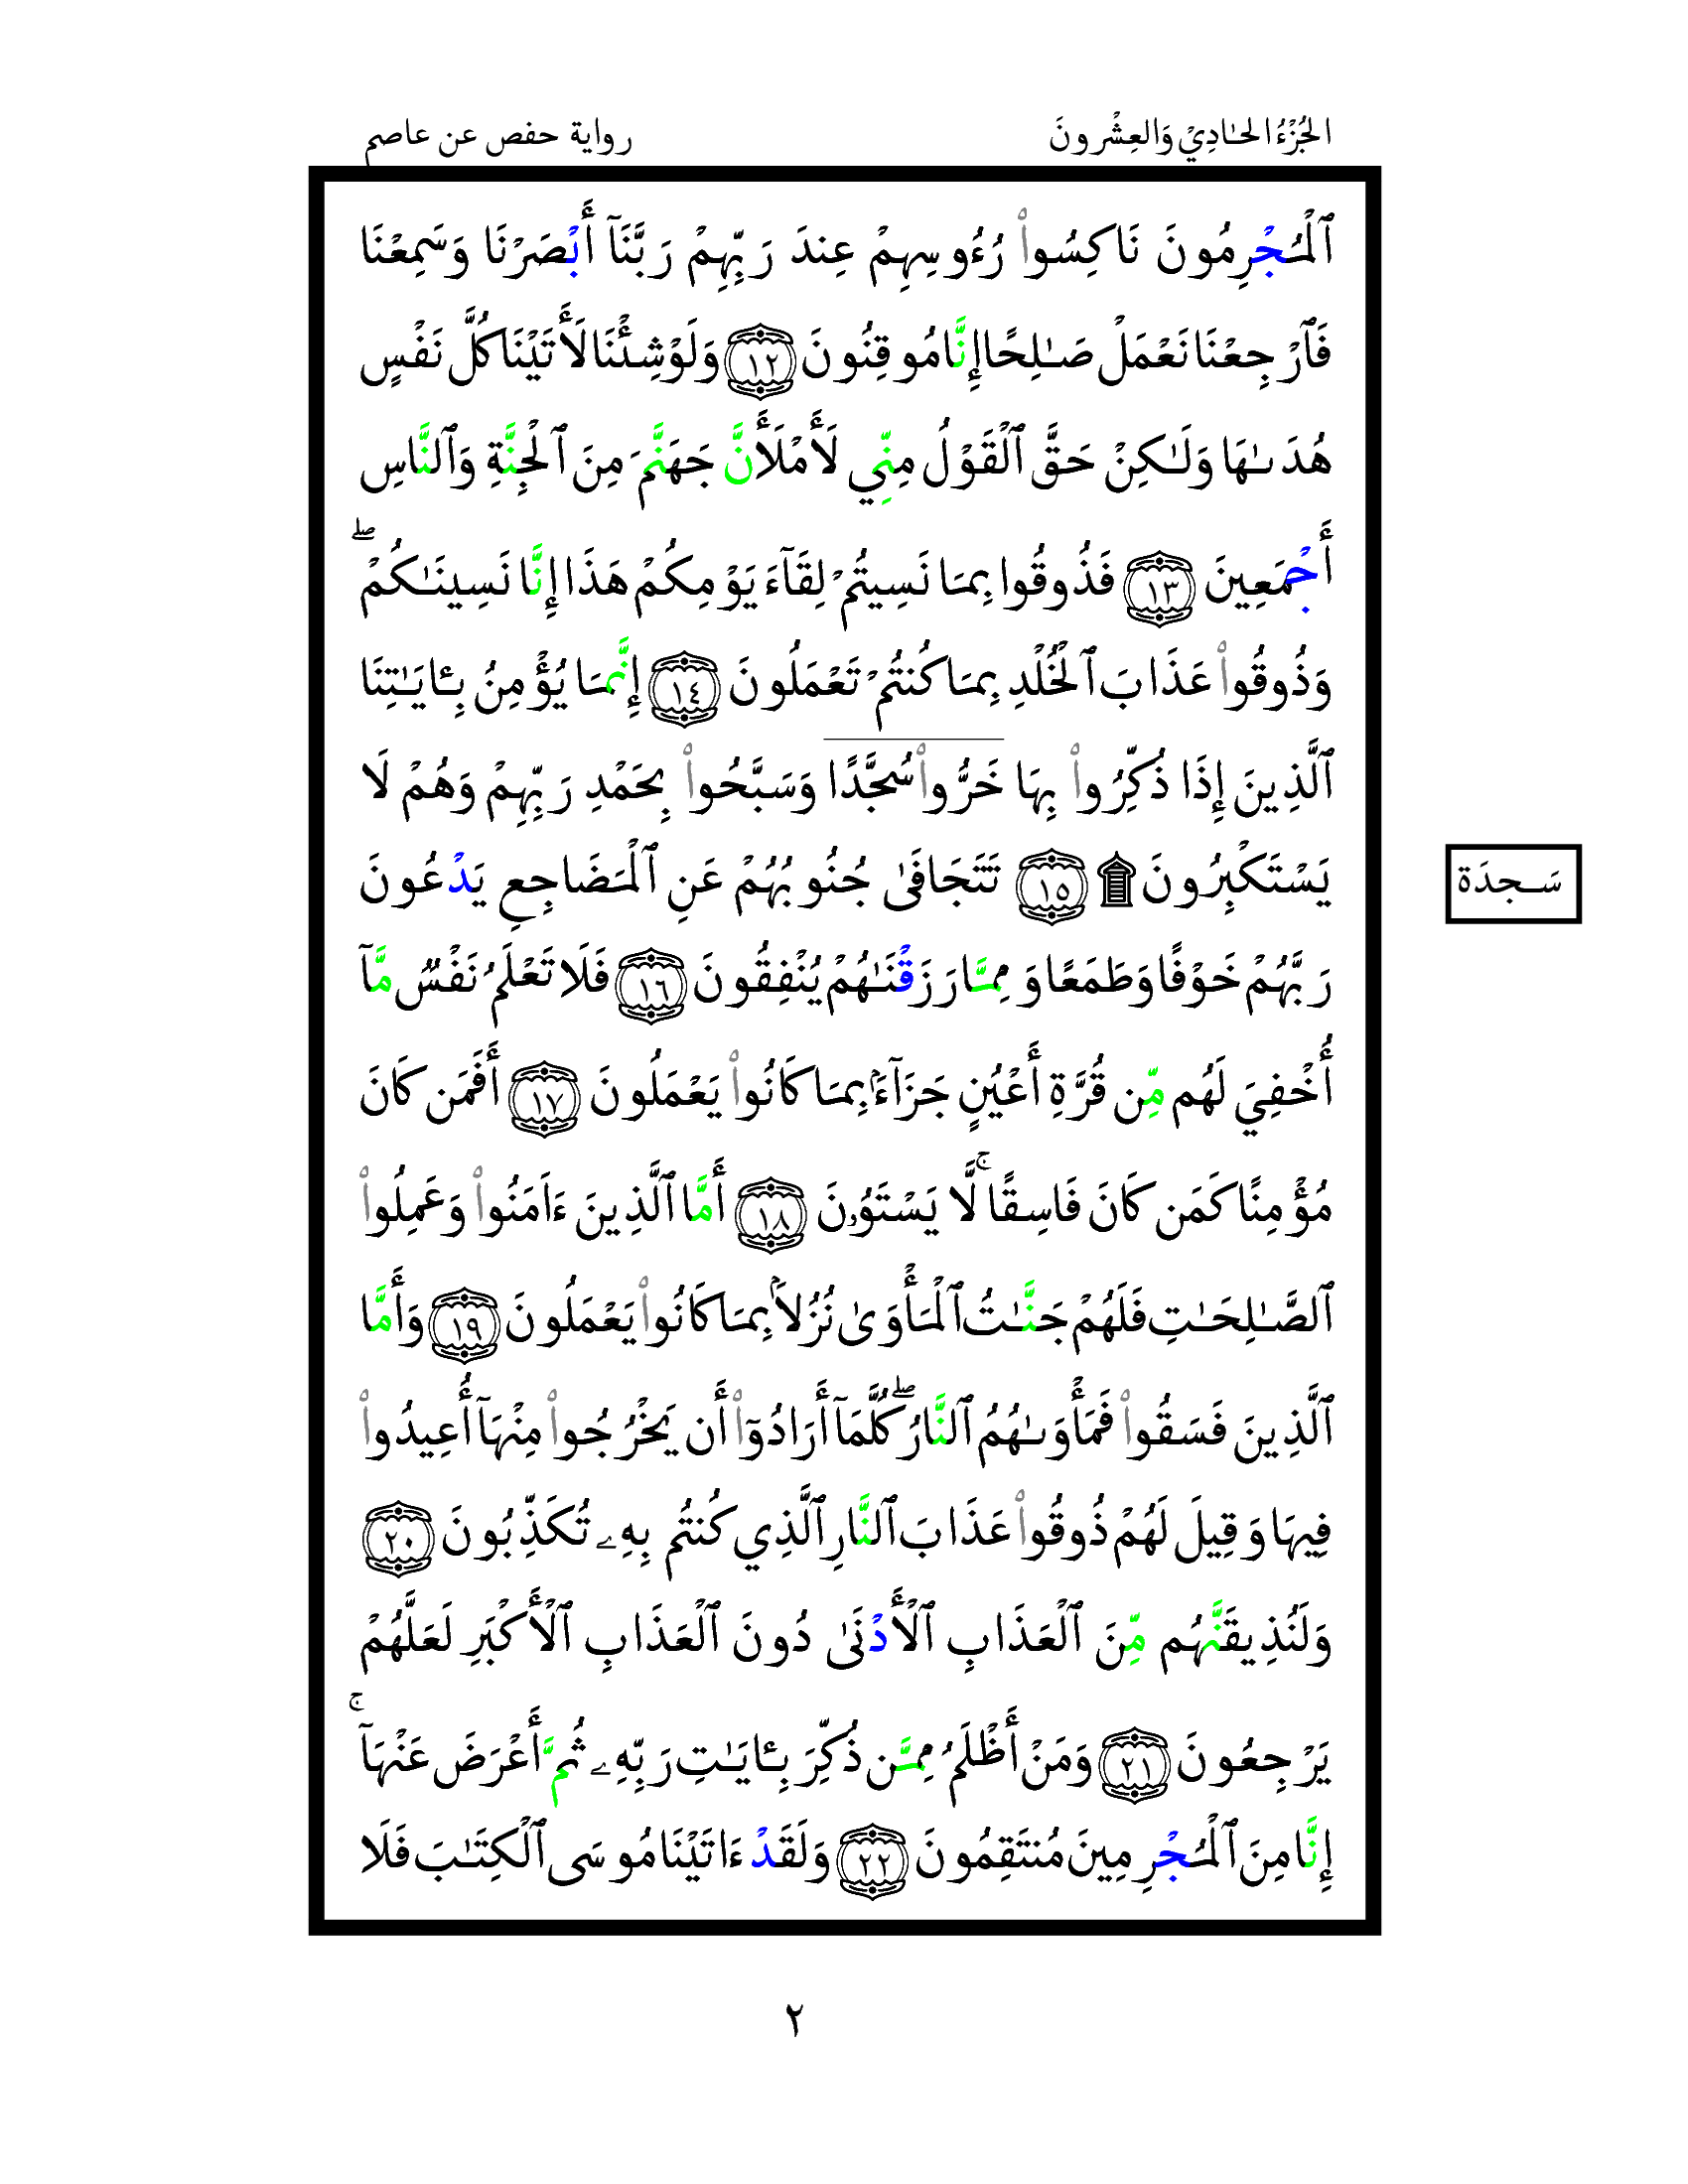
\includegraphics[scale=0.5]{sajdah_2.png}
%}
%\end{center}
%\end{minipage}
%\end{multicols}
%\end{landscape}


